\documentclass{article}
\usepackage[left=1in, right=1in, top=1in, bottom=1in]{geometry}
\usepackage{mathexam}
\usepackage{amsmath}
\usepackage{graphicx,subcaption}
\usepackage{booktabs}
\usepackage{enumitem}
\usepackage{atbegshi}% http://ctan.org/pkg/atbegshi
\usepackage[ruled,linesnumbered]{algorithm2e}
\AtBeginDocument{\AtBeginShipoutNext{\AtBeginShipoutDiscard}}

%\ExamClass{Sample Class}
%\ExamName{Sample Exam}
%\ExamHead{\today}

%\let\ds\displaystyle

\begin{document}

\begin{titlepage}
	\vspace*{\stretch{1.0}}
	\begin{center}
		\Large\textbf{Extended Experiment Report}\\
		\large\textit{December 2018}
	\end{center}
	\vspace*{\stretch{2.0}}
\end{titlepage}

%\section{Pruning performance of DiVE-Greedy and DiVE-dSwap}
%
%Note: \textit{Greedy MaxMin and Greedy Top-1 are same, both algorithms have same logic. For the rest of this report, two proposed schemes DiVE-Greedy and DiVE-dSwap will be discussed and both algorithms use Top-1 strategy.} 
%
%\subsection{DiVE-Greedy}
%Similar to the classical Greedy Construction, DiVE-Greedy initializes the set $S$ with the two most distant views.
%%
%Then, DiVE-Greedy iteratively selects new views to be added to $S$. 
%%
%Particularly, in each iteration a view is selected from the set of remaining views in $X$ and is added to $S$.
%%
%The criterion for the view that can be selected is to improve the overal hybrid objective function $F(S)$. 
%%
%Without pruning mechanism, that requires iteration of all candidate views in $X$ to find the best view that can improve $F(S)$ most. While in that process, executing query of each view is needed. 
%%
%To avoid such expensive processing, pruning scheme is proposed. 
%%
%
%\begin{figure}
%	\begin{center}
%		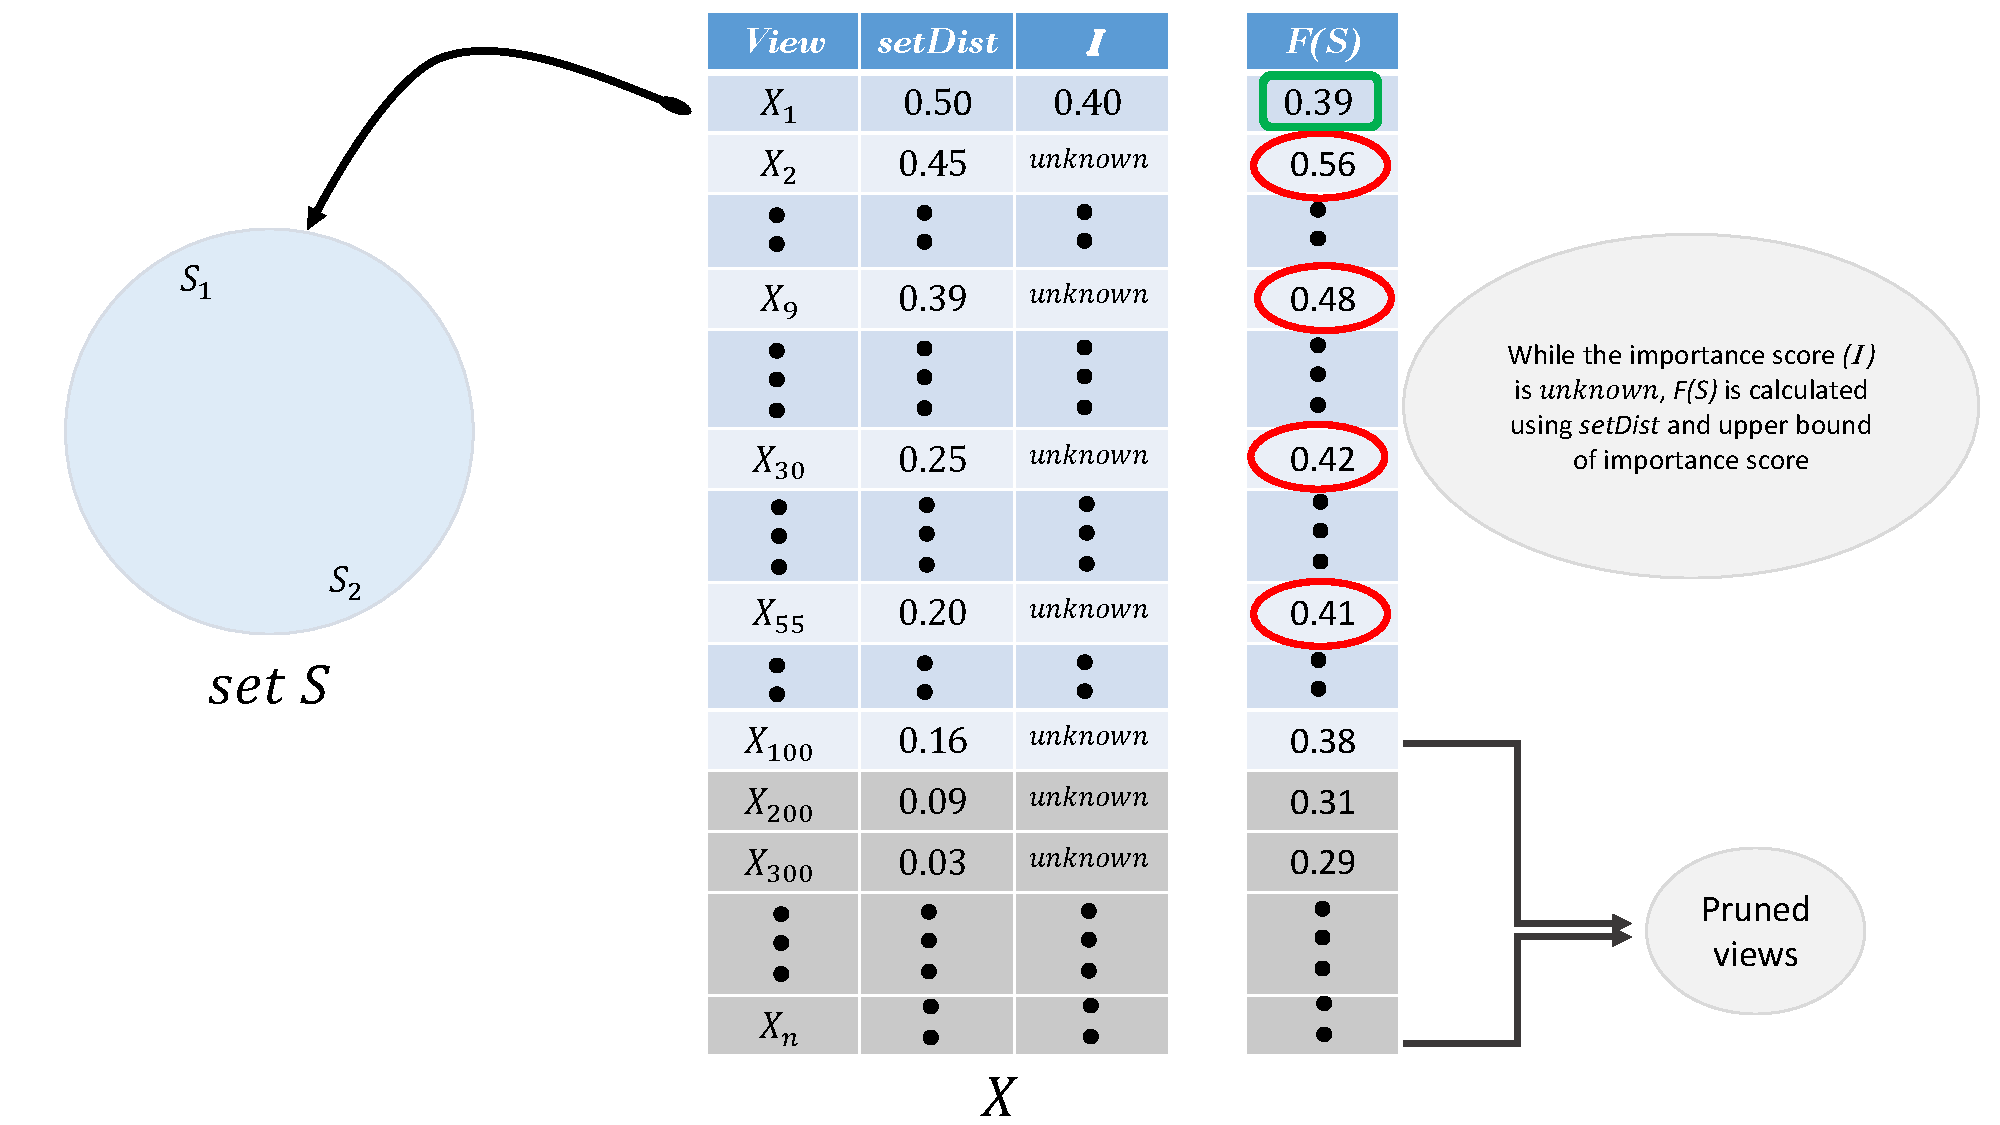
\includegraphics[width=6.0in]{figures/DiVE-Greedy}
%		\vspace{-9pt}
%		\caption{DiVE-Greedy pruning technique}
%		\label{fig:DiVE-Greedy}
%		\vspace{-20pt}
%	\end{center}
%\end{figure}
%
%Our proposed pruning technique is based on the observation that the utility score of each view $U(V_i)$ is a weighted sum of two measures; 1) the importance score of the view (i.e., $I(V_i)$), and 2) the distance of the view from $S$ (i.e., $setDist(V_i, S) $). 
%%
%We note that the computation of $setDist(V_i, S)$ is a CPU-bound (i.e., the execution time is determined by the speed of CPU). 
%%
%To the contrary, computing the importance score of a view $I(V_i)$ is an expensive operation that requires executing two queries (i.e., target and reference data) of $V_i$ (i.e., I/O-bound, where the execution time is determined by the disk speed that more slowly compared to CPU-bound).
%%
%Our pruning technique works by leveraging the diversity score and importance score that allows for pruning low-utility views without incurring the high cost for evaluating their importance as described next.
%%
%\begin{figure}
%	\begin{center}
%		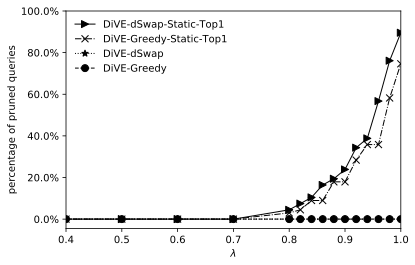
\includegraphics[width=4.0in]{figures/no_pruning_vs_static_extend}
%		\vspace{-12pt}
%		\caption{Static bound pruning performance while different value of $\lambda$, $k = 5$, MaxSum diversification function and running on Fligths dataset}
%		\label{fig:static-pruning}
%		\vspace{-20pt}
%	\end{center}
%\end{figure}
%
%
%For instance, Figure \ref{fig:DiVE-Greedy} shows how DiVE-Greedy pruning works. After the set $S$ are initialized with the two most distant views, $X$ is sorted based on the distance score of candidate views in $X$ to $S$ (i.e., $ setDist(X_i, S) $). The highest score will be on the top (i.e., the highest score of $setDist$ in this example is 0.50). Notice that up to this point there is no query execution, only diversity computation cost (i.e., $ setDist(X_i, S) $) is needed. In order to calculate the $F(S)$, the importance score of view need to be known by executing the query view. To get the importance score of the view, the query view is executed one by one starts from the top. While first view $X_1$ is executed and its importance score has been known (i.e., the importance score of $X_1$ is 0.40), the hybrid objective function can be calculated. The $F(S)$ is the objective function of set $S $ while $X_1$ is added to the set $S$ (i.e., $ F(S \cup X_1) $). This objective function will be the current objective function $ F(S) $ (i.e., 0.39). Then, $ maxF(S \cup X_i) $ of all remaining views in $X$ are calculated using actual diversity score and upper bound of importance score. 
%
%If $ maxF(S \cup X_i) < F(S) $ then it is guaranteed that the actual objective function to be less than the current objective function $ F(S) $ and these views can be pruned (i.e., all views below $X_{100}$ will be pruned). It cannot be denied because the real importance score is always below the upper bound. Meanwhile, if $ maxF(S \cup X_i) > F(S) $ such $X_2 - X_{55}$ (i.e., read circle), these views need to be executed start from the top. If on the next query view execution, there is a view that can improve $ F(S) $ compared to the current $  F(S) $, then the currect $F(S)$ will be updated. This technique is able to prune many low-quality views as shown in Figure \ref{fig:static-pruning}.
%\begin{figure}
%	\begin{center}
%%		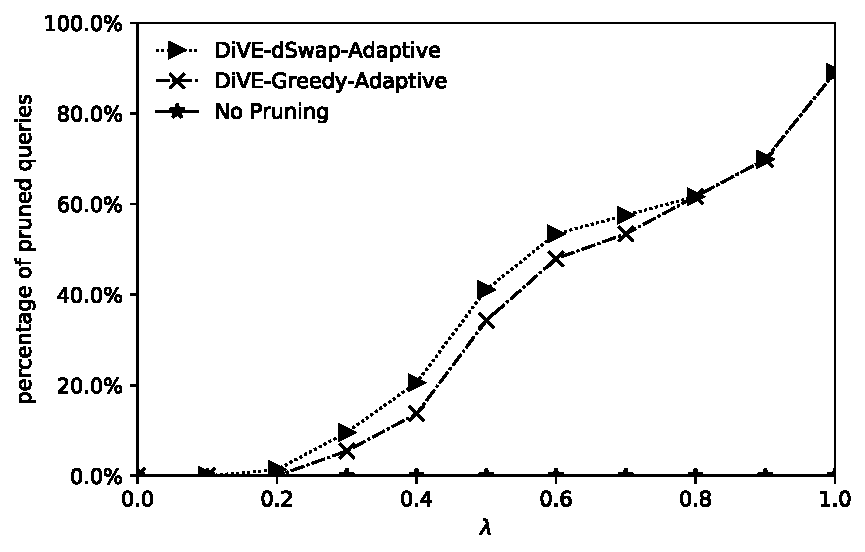
\includegraphics[width=4.0in]{figures/pruning_performance_greedy_dswap_adaptive}
%		\vspace{-12pt}
%		\caption{Adaptive bound pruning performance using different value of $ \lambda $, $k = 5$,  $ PI = 0.97 $, MaxSum diversification, running on Flights dataset}
%		\label{fig:adaptive-pruning-performance}
%		
%	\end{center}
%\end{figure}
%\subsection{DiVE-dSwap}
%As shown in the Figure \ref{fig:static-pruning}, DiVE-Greedy has a good pruning performance even it uses static bound. It will have better performance while adaptive bound is used as shown in Figure \ref{fig:adaptive-pruning-performance}. Although DiVE-Greedy is able to prune many queries, Greedy starts with small number of views (i.e., two most distant views) in the initialization set $S$ that these views cannnot be replaced. Hence, this technique may reducing the quality of recommended views in terms of effectiveness and efficiency. For instance, there is no guarantee that two most distant views which selected by Greedy as the initialization have high importance score and there is no way to replace those two views. Moreover, due to our context-driven only consist of three components (i.e., Attribute, Measure, and Aggregate Function), in the first Greedy iteration many views have same score of $ setDist(X_i, S) $ because only two views are in the set $S$. This issue may decrease the chance of pruning.
%
%In order to overcome these issues, DiVE-dSwap is proposed as well. DiVE-dSwap technique has a replacing mechanism that can replace low quality views in the current set $S$ with the better one. In addition, DiVE-dSwap has bigger number of views in the initialization set $S$ ($|S|$ = $k$). Meanwhile, higher number of views in the set $S$ can decrease the chance of views in $X$ have same $ setDist $ score.  
%
%
%In this experiment, we used Flights dataset with 5 queries, Figure \ref{fig:static-pruning} shows the pruning performance of DiVE-Greedy and DiVE-dSwap while static bound is used and Figure \ref{fig:adaptive-pruning-performance} while adaptive bound is used. 
%




\section{Context-Driven Distance Functions}

Jaccard similarity and cosine similarity are two very common measurements while comparing item similarities. Similarity measures are used in various ways, examples include in plagiarism, collaborative filtering in recommendation systems, and etc. 

Jaccard similarity is given by $$J(A, B) = \frac{|A \cap B|}{|A \cup B|} = \frac{|A \cap B|}{|A \cap B| + |A - B| + |B - A|}$$

Cosine similarity is given by $$C(A, B) = \frac{|A \cap B|}{\sqrt{\left|A\right|\left|B\right|}} = \frac{|A \cap B|}{\sqrt{(\left|A\cap B\right| + |A - B|)(\left|A\cap B\right| + |B - A|)}}$$

Simply put, in cosine similarity, the number of common attributes is divided by the total number of possible attributes. Whereas in Jaccard Similarity, the number of common attributes is divided by the number of attributes that exists in at least one of the two objects. 

In our experiment, we implemented both distances. Based on our result, the Jaccard distance can perform better compare to Cosine distance in terms of pruning performance. Here why Jaccard has better performance in our work, for instance, given two views which are A = ['chest\_pain\_types', 'oldpeak', 'avg'] and B = ['chest\_pain\_types', 'thal', 'max']. Similarity score of A and B is 0.3333 by Cosine similarity and 0.166666 by Jaccard similarity. Our work focus on dissimilarity between views. If disimilarity can be calcualte by $1 - Similarity\ Score$, then the distance score of A and B is 0.667 by Cosine dissimilarity and 0.833 by Jaccard dissimilarity.

The result shows that Jaccard distance has higher dissimilarity score compare to Cosine distance. Hence, using Jaccard distance function makes the schemes has better performance in terms of pruning rather than using Cosine distance function.  
\\


\noindent{\textit{Note: 1 - Jaccard Coefficient can be used as a dissimilarity or distance measure, whereas the cosine similarity has no such constructs.}} I am not sure how to calculate dissimilarity score using Cosine similarity. 


\section{Prediction Interval}


We decide to rely on non-parametric predictive interval models to determine maximum value with certain level of confidence. However, nonparametric methods are most appropriate when the sample sizes are small. When the dataset is large (e.g., N $>$ 1000) it often makes no sense to use nonparametric method. 

In case of the large dataset, we can use parametric method with the equation as follows:


$s = (X^2 NP(1-P)) / (d^2 (N -1) + X^2 P(1-P)) $, 

\noindent Where: 

$s$ = required sample size. 

$X^2$ = the table value of chi-square for 1 degree of freedom at the desired confidence level (3.841).

$N$ = the population size. 

$P$ = the population proportion (assumed to be 0.5 since this would provide the maximum sample size). 

$d$ = the degree of accuracy expressed as a proportion (0.5)

\noindent The table detail of determining sample size from a given population can be seen on the link below \footnote{https://journals.sagepub.com/doi/abs/10.1177/001316447003000308}. 


\section{Hierarchical Attributes}

\begin{figure}%
	\centering
	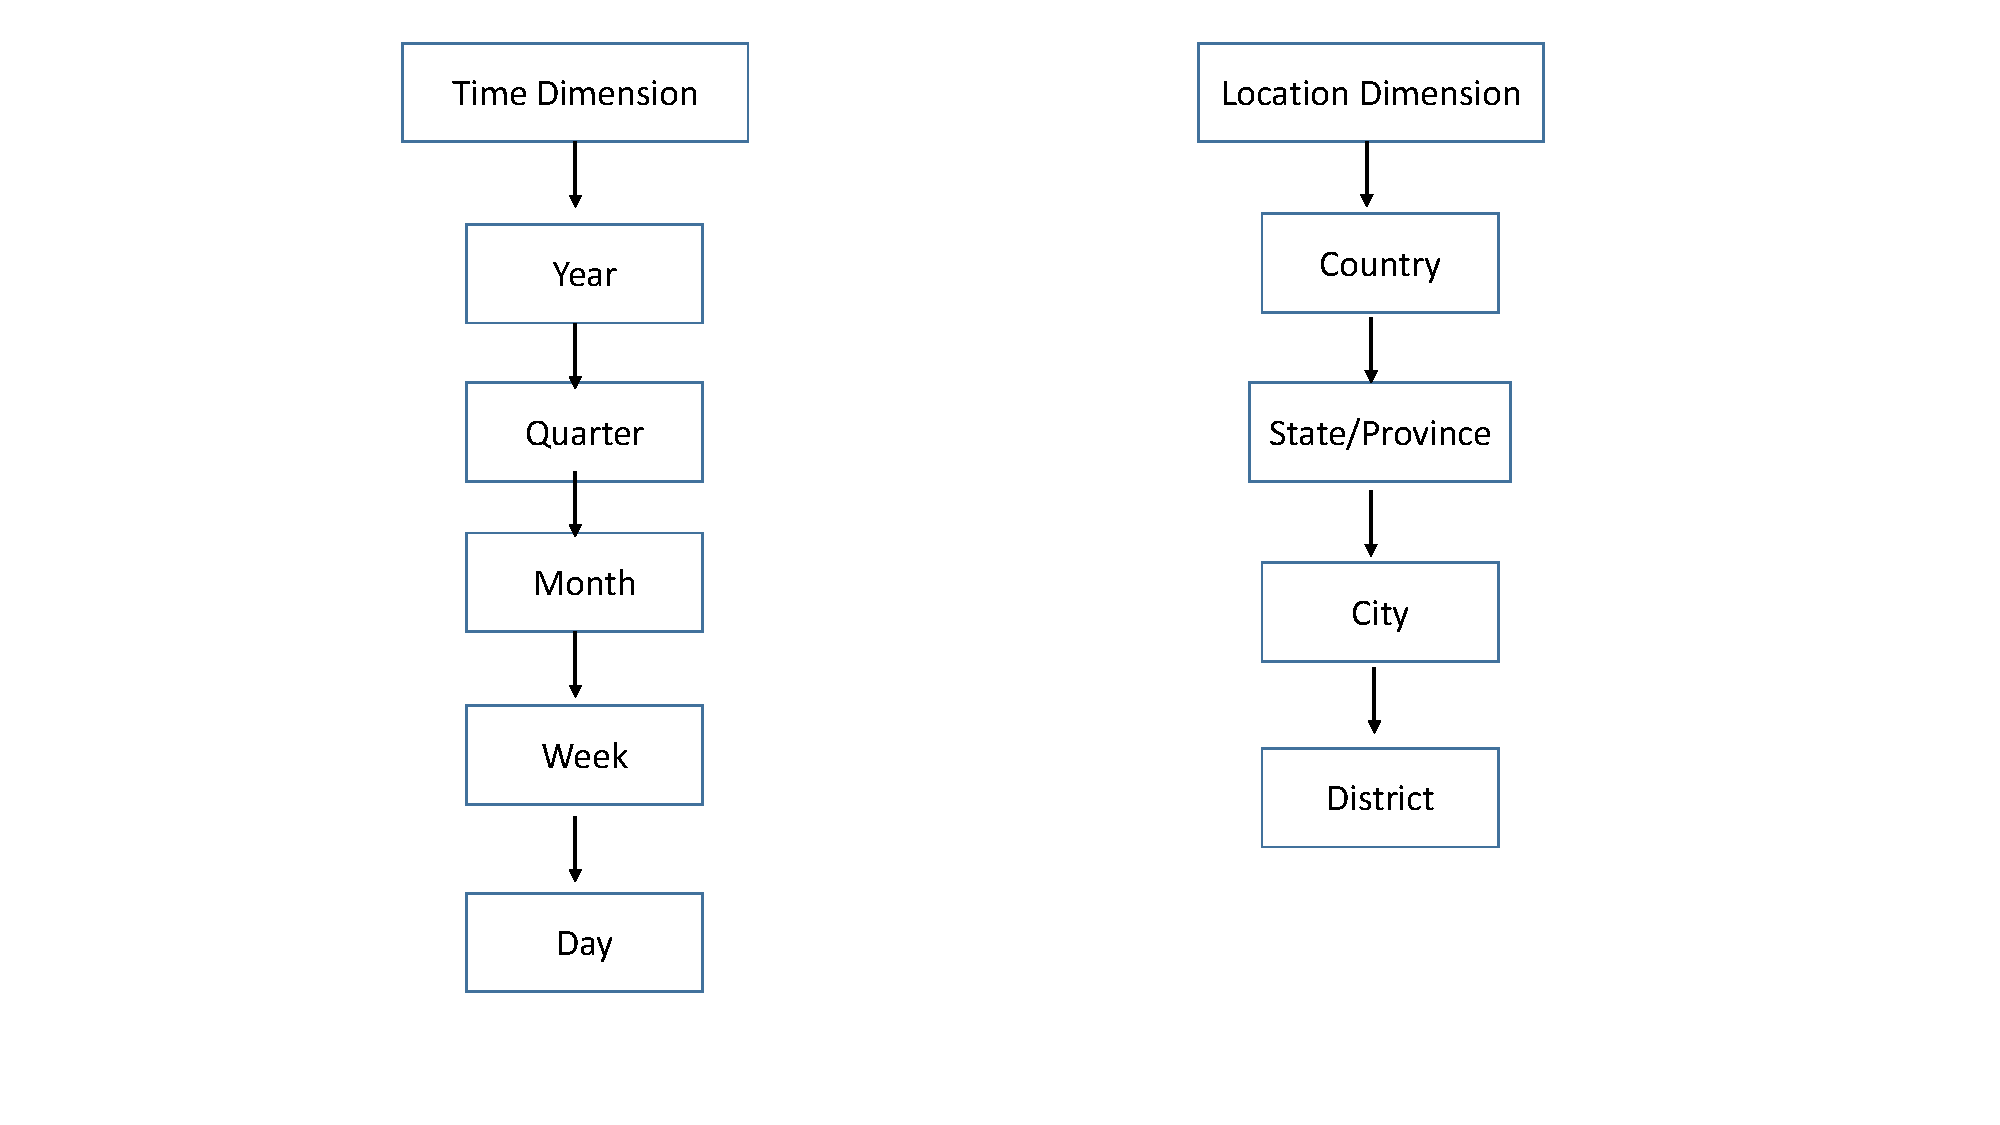
\includegraphics[width=5.2in]{figures/hirarki_atribut}
	\caption{An example of hierarchical attribute}
	\label{fig:hierarchial_attribute}%
\end{figure}


The dataset contains such as location dimensions (country, state, province, city), time dimensions (Year, Quarter, Week, Days), product dimensions (product categories) as shown in Figure \ref{fig:hierarchial_attribute} commonly can be processed by OLAP. We need to find a way to calculate the similarity and dissimilarity between two views which have hierarchical attributes.
\\

\noindent{Given an example OLAP query as follows: }
\begin{verbatim}
SELECT QUARTER, REGION, SUM(SALES)
FROM SALESTABLE
GROUP BY (QUARTER)
\end{verbatim}

According to Figure \ref{fig:hierarchial_attribute}, this query has two hierarchical attributes which are $QUARTER$ and $REGION$. There are several previous works which focus on measuring similairity between OLAP's queries. Such as in the example above, OLAP query usually has more than one hierarchical attributes. However, in our work, the view will never has more than one hierarchical attributes. A view in our works consists only three components (one categorical attribute, one numerical attribute, and one aggregate function). To the best of our knowledge, only categorical attribute that can possibly has a hierarchy. 

The main issue in our work is how to compute the distance between two views which have hierarchical attributes. For instance, given two views: $A [year, sales, avg]$ and $B [month, sales, avg]$. Without considering hierarchy the distance value between $year$ and $month$ is 1 (0 if same and 1 if different). However, by considering hierarchy we can have different distance score. 

A simple way is to use height parameter. For instance, as shown in Figure \ref{fig:hierarchial_attribute}, time dimension has 5 levels (height). Given two views: $A [year, sales, avg]$ and $B [month, sales, avg]$, the distance between $year$ and $month$ is $\frac{|H(V_i) - H(V_j)|}{Len(H)}$ =  $ \frac{|1 - 3|}{5} $ = $\frac{2}{5}$. While the categorical attribute from both view is exactly same, the distance is 0, e.g., $year$ vs. $year$ =  $ \frac{|1 - 1|}{5} $ = 0.


\begin{figure}%
	\centering
	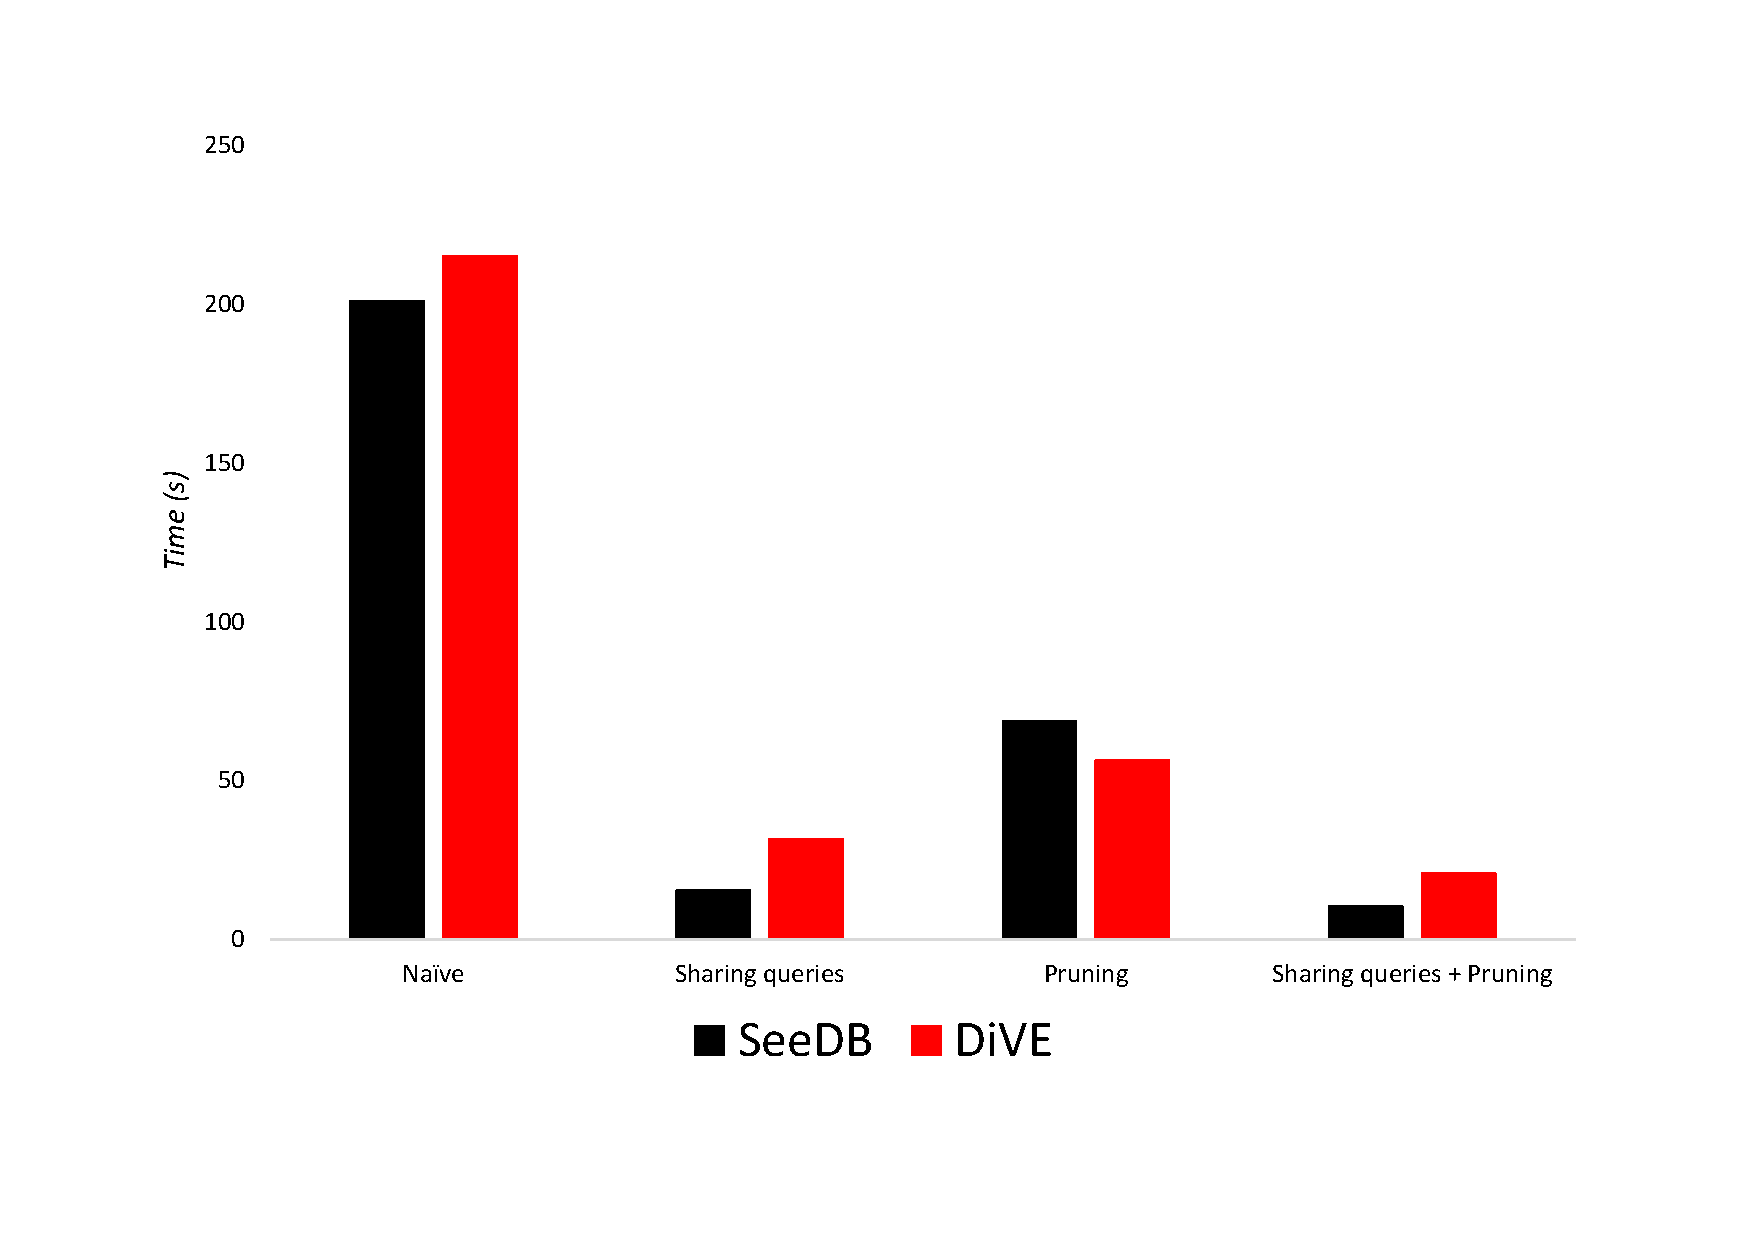
\includegraphics[width=5.2in]{figures/SeeDB_vs_DiVE}
	\caption{Performance comparision of SeeDB and DiVE with sharing queries optimization and pruning}
	\label{fig:SeeDB_vs_DiVE}%
\end{figure}
\section{Costs Reduction}

\subsection{SeeDB vs. DiVE}
\subsubsection{Naive Search}
We implemented a SeeDB naive exhaustive search by looping over all possible combinations of attributes,  measure attributes, and aggregation functions where all queries are executed and no pruning required. DiVE naive search is implemented in the same way as SeeDB in terms of query execution. In this experiment, the only different between SeeDB and DiVE is DiVE has a diversification.

%There are two types of exhaustive implementation which are: 1) without combine target and reference query 2) combining target and reference query. 





\subsubsection{Pruning optimizations}
One way to further speed up the processing to find the top-k views, is to not evaluate queries with a low likelihood of being in the list of top-k most interesting views. We implemented pruning optimizations based on the paper. We splited the data into N phases (for example: N=15), then for each view currently being considered, we compute the importance score of that view on that partition. We then find the mean of the partition importance score thus far evaluated, and compute a confidence interval around that mean. If the upper-bound of the confidence interval for a view is lower than the lower-bound of the top-k views, then we drop that view from consideration. On the other hand, DiVE utilizes importance and diversity score to prune low-quality views. In this experiment, we used $\lambda = 0.6$ and $PI 90$.


\subsubsection{Query sharing optimizations}
We followed the SeeDB paper that the autors applied sharing optimization by combining the queries with the same group-by attributes to perform multiple aggregations. This results in the execution of just two queries for every new group by attribute.

The version of published DiVE scheme used pruning as the way to reduce the costs. In this experiment, we applied query sharing on DiVE. Instead of executing query views start from the top directly, DiVE collected some views with same group-by and performing multiple aggregations. 

%For the confidence interval, the paper uses a result derived from the Hoeffding-Serfling inequality. If we have a set of data $\{X_1, X_2, ..., X_n\}$ and sample from that with m samples $\{x_1, x_2, ..., x_m\}$, then the mean of our samples $x_m$ will be within $\epsilon$ of the true mean with probability $(1-\delta)$. In our case, the set of data $y_N$ is the utility of each of the 15 partitions, and each sample $Y_m$ is one of the thus far evaluated partitions. Becuase the Hoeffding-Serfling inequality is defined over values between 0 and 1, we normalize our sample means by dividing them all by the max mean utility value. This ensures that all values will be in the allowed range. We use a $\delta$ of 0.1, leading to a confidence interval epsilon where our sample mean is 90\% likely to be within $\epsilon$ of the true mean.

\subsubsection{Cost comparison result}
\textit{\textbf{\noindent{SeeDB}}}. The naive exhaustive search method of SeeDB has a runtime of 201 seconds.
When we implement the sharing-based multiple aggregation optimizations, we get a runtime of 15.375 seconds, for a speedup of 13x. By using pruning optimizations on the naive method, we get a runtime of 68.6 seconds for a 2.9x speedup. Implementing both optimizations gives us a runtime of 10.4 seconds for a speedup of 19x over exhaustive search. 

\noindent{\textbf{\textit{DiVE}}}. The total cost of DiVE naive search is 215 seconds. DiVE with adaptive pruning has a runtime of 56.26 seconds for a 3.8x speedup. Implement the sharing-based multiple aggregation optimizations on DiVE, we get speedup of 6.8x (37.57 seconds). While we implementing both optimizations gives us a runtime of 20.65 seconds for a speedup of 10.5x over exhaustive search. 

These experiments were conducted on a Windows Dell with 3.6 GHz Intel Core i7-7700 and using Flights dataset. The detail comparison can be seen in Figure \ref{fig:SeeDB_vs_DiVE}. Overall, the performance of DiVE is below SeeDB due to DiVE has diversity function that need to be calculated. Moreover, combining both optimizations (pruning and query sharing) give us optimum performance for both SeeDB and DiVE. 







\section{New Dataset}

The student performance dataset is used in this experiment as the motivation example dataset. This dataset can be downloaded from Kaggle \footnote{https://www.kaggle.com/uciml/student-alcohol-consumption} and UCI ML website \footnote{https://archive.ics.uci.edu/ml/datasets/student+performance}. This dataset has 28 attributes, 5 measures, and four aggregate functions are used in this experiments. The data were obtained in a survey of students math and Portuguese language courses in secondary school. It contains a lot of interesting social, gender and study information about students. In this experiment, only math dataset is used. 

For instance, the analyst wants to compare between students who want to continue their study to the higher education and students who do not want to continue their study to higher education. Figure \ref{fig:motivation_dataset} shows two views that have the highest importance score: 1) A = studytime, M = final grade, and F = AVG, the importance score is 0.812831582477977; 2) A = studytime, M = final grade, and F = MAX, the importance score is 0.797221012363291. This Figure shows without diversity, recommended views may suffer from redundancy. 


Figure \ref{fig:motivation_dataset} also describes that students who want to continue to higher education relatively have better final grade compared to students who do not want to continue to higher education. Interestingly, some students who want to continue their education, they spend more time to study (5 to 10 hours, even more than 10 hours) per week. To contrary, students who do not want to continue their study, all of them only spend less than 5 hours a week for study.


\begin{figure}%
	\centering
	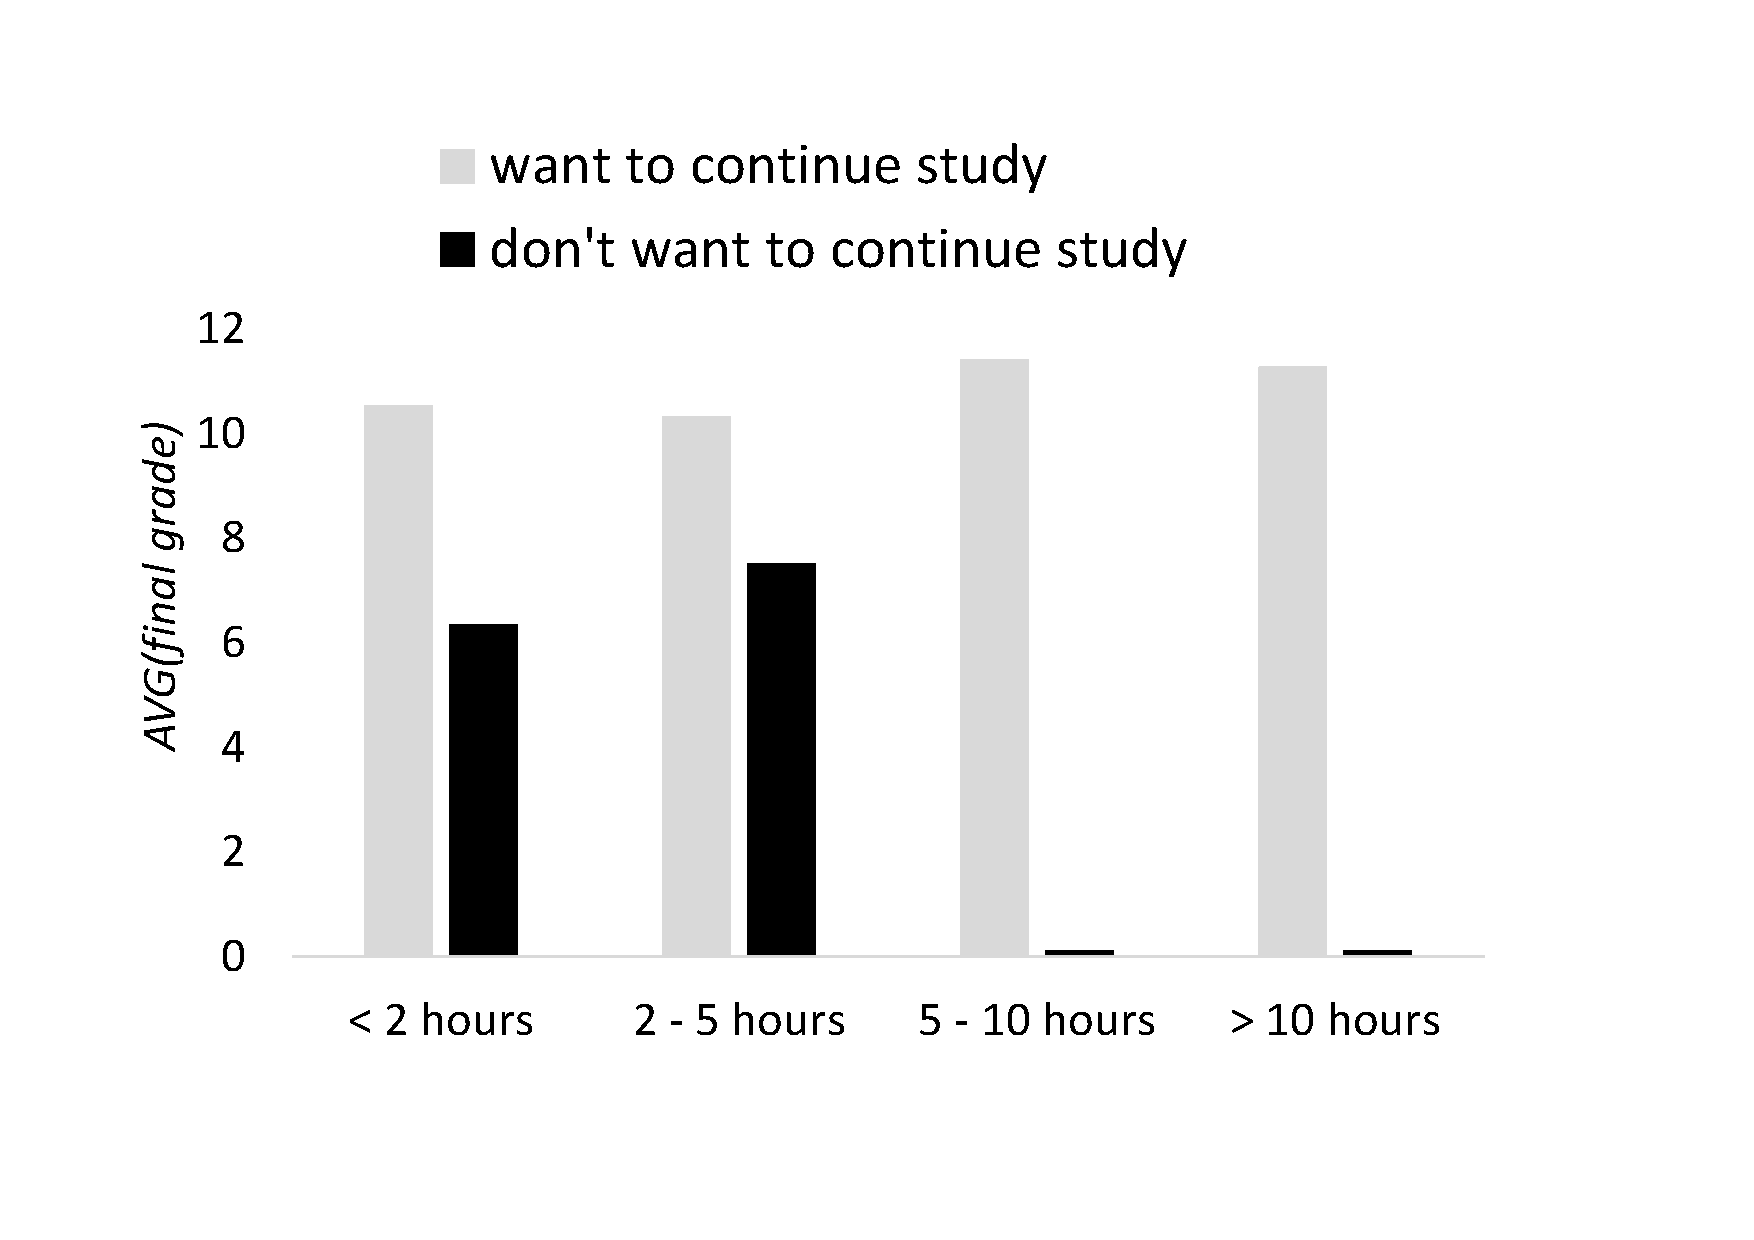
\includegraphics[width=3.2in]{figures/AVG_STUDENT}
	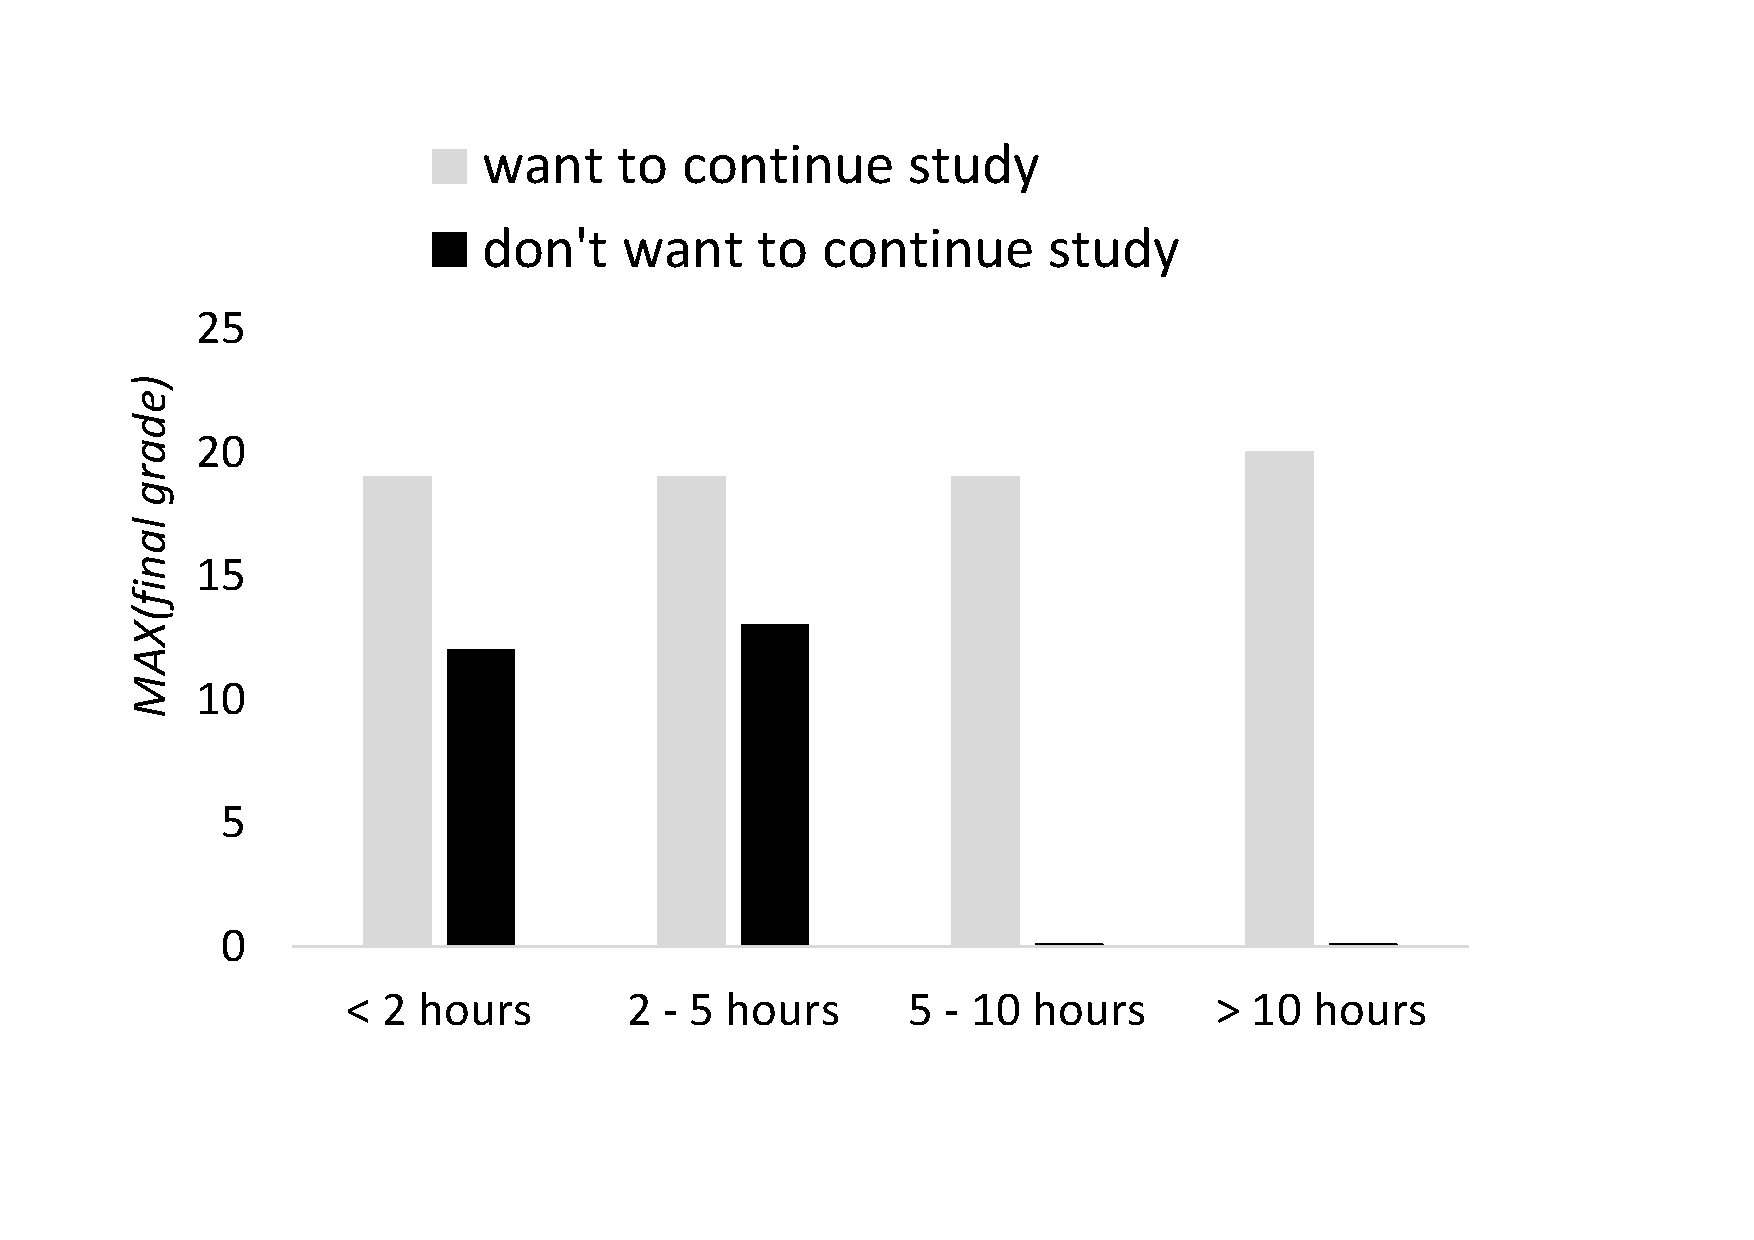
\includegraphics[width=3.2in]{figures/MAX_STUDENT}
	\caption{Study time and final grade of students who want to countinue their study to higher education vs. students who do not want to continue their study to higher education}%
	\label{fig:motivation_dataset}%
\end{figure}

\end{document}
